\documentclass{standalone}
\usepackage{tikz}
\usetikzlibrary{patterns, positioning}
\usepackage[sfdefault]{ClearSans} %% option 'sfdefault' activates Clear Sans as the default text font
\usepackage[T1]{fontenc}

\begin{document}
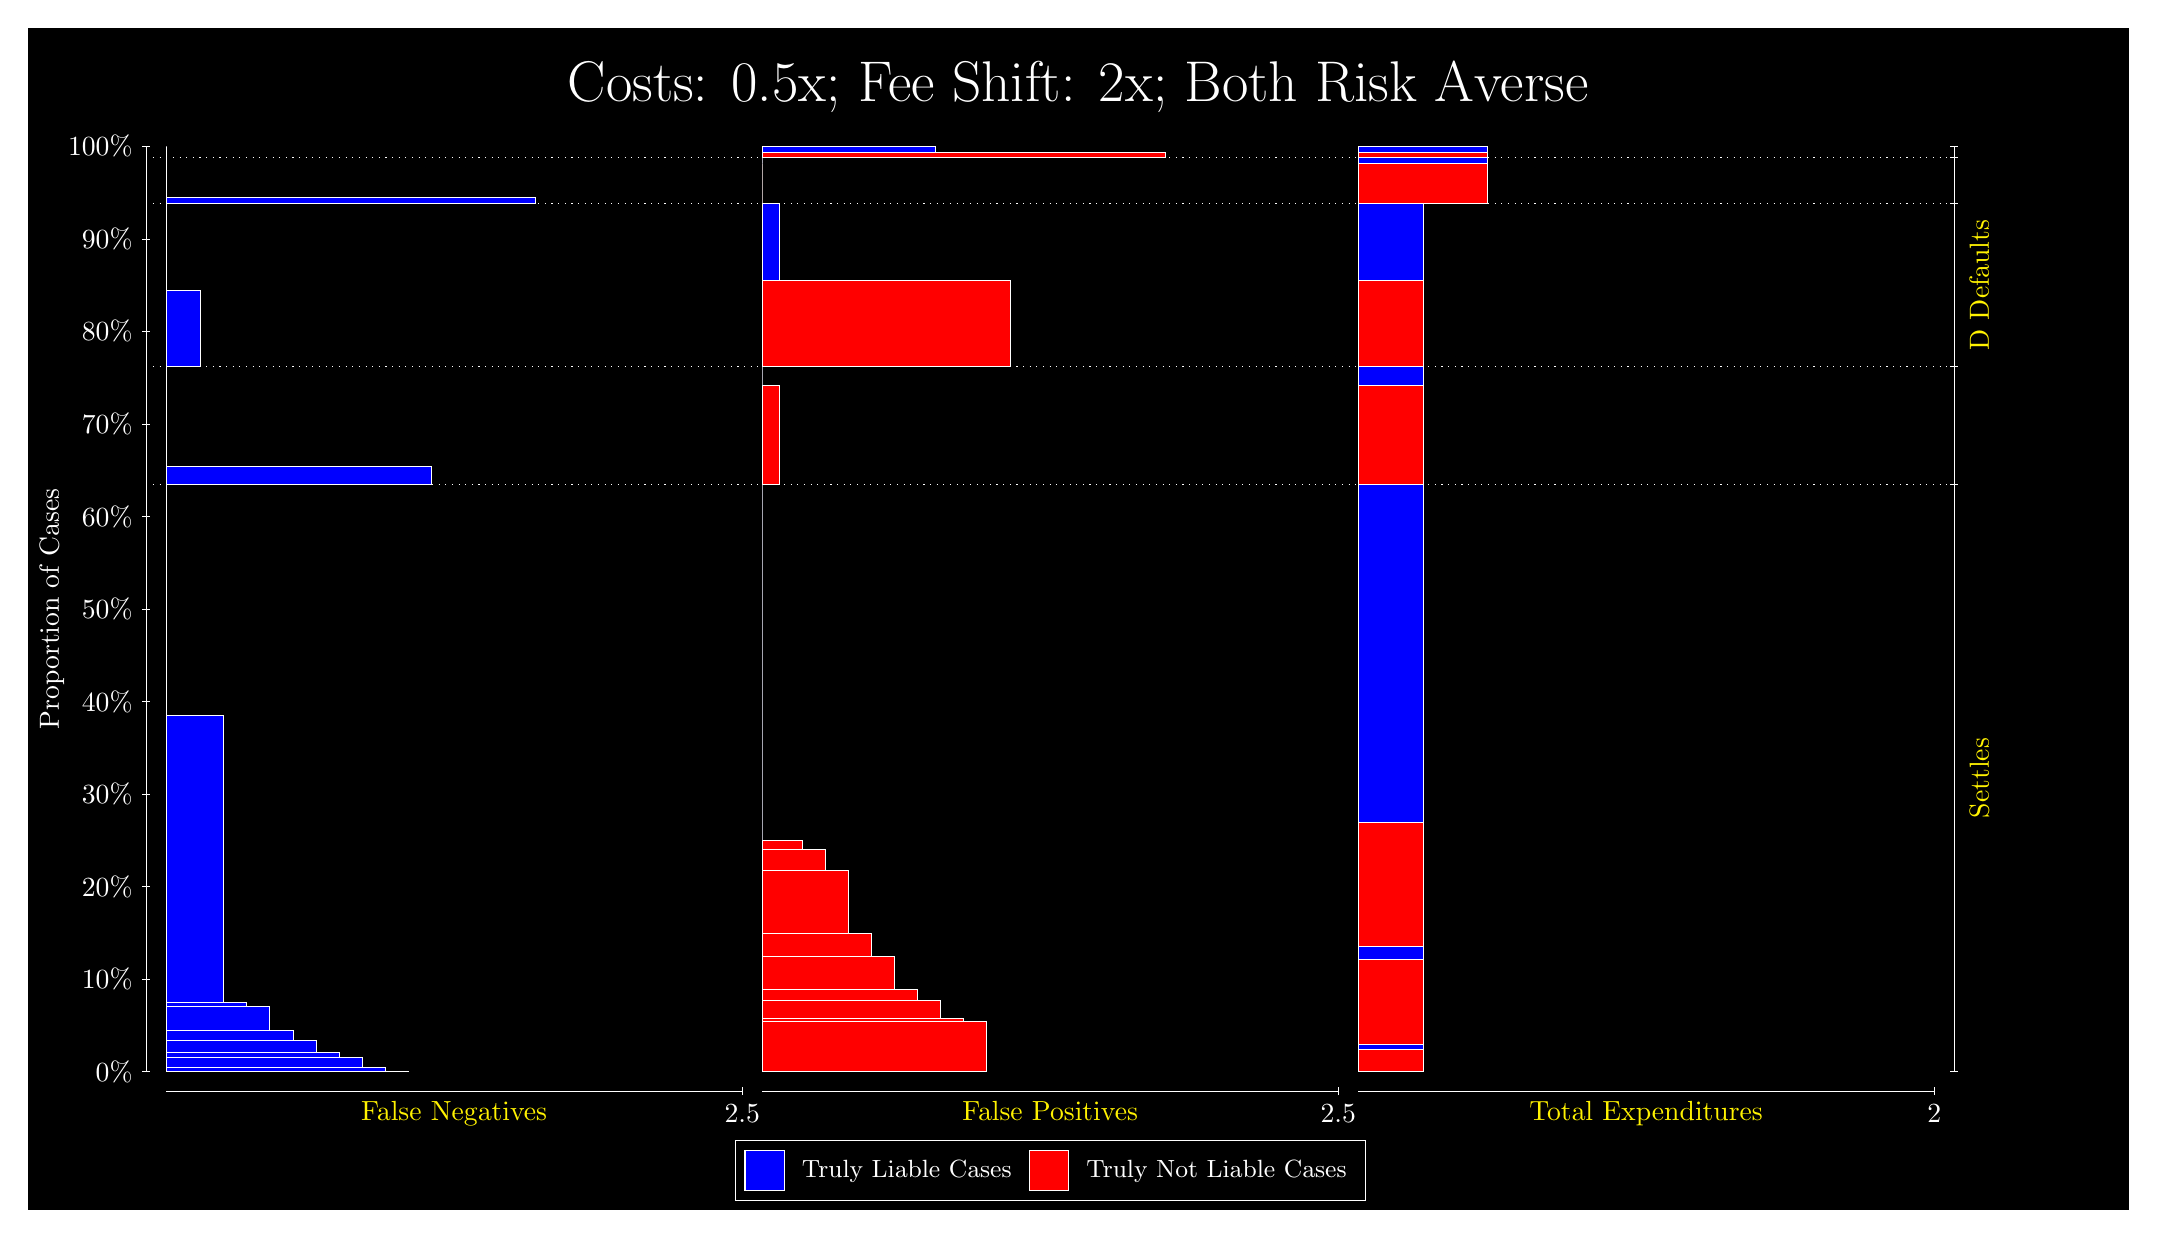
\begin{tikzpicture}
\draw[fill=black] (0,0) rectangle (26.667,15);
\draw[text=white] (0,13.5) rectangle (26.667,15) node[midway] {\huge Costs: 0.5x; Fee Shift: 2x; Both Risk Averse};
\draw[white, very thin] (1.5,1.75) -- (1.5,13.5);
\node[rotate=90, text=white, anchor=center] at (0.3, 7.625) {Proportion of Cases};
\draw[white, very thin] (1.45,1.75) -- (1.55,1.75);
\node[text=white, anchor=east] at (1.45, 1.75) {0\%};
\draw[white, very thin] (1.45,2.925) -- (1.55,2.925);
\node[text=white, anchor=east] at (1.45, 2.925) {10\%};
\draw[white, very thin] (1.45,4.1) -- (1.55,4.1);
\node[text=white, anchor=east] at (1.45, 4.1) {20\%};
\draw[white, very thin] (1.45,5.275) -- (1.55,5.275);
\node[text=white, anchor=east] at (1.45, 5.275) {30\%};
\draw[white, very thin] (1.45,6.45) -- (1.55,6.45);
\node[text=white, anchor=east] at (1.45, 6.45) {40\%};
\draw[white, very thin] (1.45,7.625) -- (1.55,7.625);
\node[text=white, anchor=east] at (1.45, 7.625) {50\%};
\draw[white, very thin] (1.45,8.8) -- (1.55,8.8);
\node[text=white, anchor=east] at (1.45, 8.8) {60\%};
\draw[white, very thin] (1.45,9.975) -- (1.55,9.975);
\node[text=white, anchor=east] at (1.45, 9.975) {70\%};
\draw[white, very thin] (1.45,11.15) -- (1.55,11.15);
\node[text=white, anchor=east] at (1.45, 11.15) {80\%};
\draw[white, very thin] (1.45,12.325) -- (1.55,12.325);
\node[text=white, anchor=east] at (1.45, 12.325) {90\%};
\draw[white, very thin] (1.45,13.5) -- (1.55,13.5);
\node[text=white, anchor=east] at (1.45, 13.5) {100\%};

\draw[white, very thin] (24.457,1.75) -- (24.457,13.5);
\draw[white, very thin] (24.407,1.75) -- (24.507,1.75);
\node[anchor=west] at (24.407, 1.75) {};
\draw[white, very thin] (24.407,9.2044) -- (24.507,9.2044);
\node[anchor=west] at (24.407, 9.2044) {};
\draw[white, very thin] (24.407,10.701) -- (24.507,10.701);
\node[anchor=west] at (24.407, 10.701) {};
\draw[white, very thin] (24.407,12.775) -- (24.507,12.775);
\node[anchor=west] at (24.407, 12.775) {};
\draw[white, very thin] (24.407,13.356) -- (24.507,13.356);
\node[anchor=west] at (24.407, 13.356) {};
\draw[white, very thin] (24.407,13.5) -- (24.507,13.5);
\node[anchor=west] at (24.407, 13.5) {};

\draw[white, very thin, fill=blue] (1.75,1.75) rectangle (4.8239,1.7593);
\draw[white, very thin, fill=blue] (1.75,1.7593) rectangle (4.5312,1.8004);
\draw[white, very thin, fill=blue] (1.75,1.8004) rectangle (4.2384,1.9323);
\draw[white, very thin, fill=blue] (1.75,1.9323) rectangle (3.9457,1.9956);
\draw[white, very thin, fill=blue] (1.75,1.9956) rectangle (3.6529,2.1532);
\draw[white, very thin, fill=blue] (1.75,2.1532) rectangle (3.3602,2.2692);
\draw[white, very thin, fill=blue] (1.75,2.2692) rectangle (3.0674,2.5838);
\draw[white, very thin, fill=blue] (1.75,2.5838) rectangle (2.7746,2.63);
\draw[white, very thin, fill=blue] (1.75,2.63) rectangle (2.4819,6.2704);
\draw[white, very thin, fill=red] (1.75,6.2704) rectangle (1.75,9.2044);
\draw[white, very thin, fill=blue] (1.75,9.2044) rectangle (5.1167,9.4406);
\draw[white, very thin, fill=red] (1.75,9.4406) rectangle (1.75,10.701);
\draw[white, very thin, fill=blue] (1.75,10.701) rectangle (2.1891,11.673);
\draw[white, very thin, fill=red] (1.75,11.673) rectangle (1.75,12.775);
\draw[white, very thin, fill=blue] (1.75,12.775) rectangle (6.4341,12.849);
\draw[white, very thin, fill=red] (1.75,12.849) rectangle (1.75,13.356);
\draw[white, very thin, fill=red] (1.75,13.356) rectangle (1.75,13.428);
\draw[white, very thin, fill=blue] (1.75,13.428) rectangle (1.75,13.5);
\draw[white, very thin, fill=red] (9.3189,1.75) rectangle (12.173,2.3861);
\draw[white, very thin, fill=red] (9.3189,2.3861) rectangle (11.88,2.4274);
\draw[white, very thin, fill=red] (9.3189,2.4274) rectangle (11.588,2.6526);
\draw[white, very thin, fill=red] (9.3189,2.6526) rectangle (11.295,2.8009);
\draw[white, very thin, fill=red] (9.3189,2.8009) rectangle (11.002,3.2189);
\draw[white, very thin, fill=red] (9.3189,3.2189) rectangle (10.709,3.5063);
\draw[white, very thin, fill=red] (9.3189,3.5063) rectangle (10.709,3.5089);
\draw[white, very thin, fill=red] (9.3189,3.5089) rectangle (10.417,4.3098);
\draw[white, very thin, fill=red] (9.3189,4.3098) rectangle (10.124,4.5789);
\draw[white, very thin, fill=red] (9.3189,4.5789) rectangle (9.8312,4.6839);
\draw[white, very thin, fill=blue] (9.3189,4.6839) rectangle (9.3189,9.2044);
\draw[white, very thin, fill=red] (9.3189,9.2044) rectangle (9.5384,10.465);
\draw[white, very thin, fill=blue] (9.3189,10.465) rectangle (9.3189,10.701);
\draw[white, very thin, fill=red] (9.3189,10.701) rectangle (12.466,11.803);
\draw[white, very thin, fill=blue] (9.3189,11.803) rectangle (9.5384,12.775);
\draw[white, very thin, fill=red] (9.3189,12.775) rectangle (9.3189,13.281);
\draw[white, very thin, fill=blue] (9.3189,13.281) rectangle (9.3189,13.356);
\draw[white, very thin, fill=red] (9.3189,13.356) rectangle (14.442,13.428);
\draw[white, very thin, fill=blue] (9.3189,13.428) rectangle (11.515,13.5);
\draw[white, very thin, fill=red] (16.888,1.75) rectangle (17.711,2.0374);
\draw[white, very thin, fill=blue] (16.888,2.0374) rectangle (17.711,2.0999);
\draw[white, very thin, fill=red] (16.888,2.0999) rectangle (17.711,3.1724);
\draw[white, very thin, fill=blue] (16.888,3.1724) rectangle (17.711,3.3462);
\draw[white, very thin, fill=red] (16.888,3.3462) rectangle (17.711,4.9202);
\draw[white, very thin, fill=blue] (16.888,4.9202) rectangle (17.711,9.2044);
\draw[white, very thin, fill=red] (16.888,9.2044) rectangle (17.711,10.465);
\draw[white, very thin, fill=blue] (16.888,10.465) rectangle (17.711,10.701);
\draw[white, very thin, fill=red] (16.888,10.701) rectangle (17.711,11.803);
\draw[white, very thin, fill=blue] (16.888,11.803) rectangle (17.711,12.775);
\draw[white, very thin, fill=red] (16.888,12.775) rectangle (18.534,13.281);
\draw[white, very thin, fill=blue] (16.888,13.281) rectangle (18.534,13.356);
\draw[white, very thin, fill=red] (16.888,13.356) rectangle (18.534,13.428);
\draw[white, very thin, fill=blue] (16.888,13.428) rectangle (18.534,13.5);
\draw[white, dotted] (1.5,9.2044) -- (24.457,9.2044);
\draw[white, dotted] (1.5,10.701) -- (24.457,10.701);
\draw[white, dotted] (1.5,12.775) -- (24.457,12.775);
\draw[white, dotted] (1.5,13.356) -- (24.457,13.356);
\draw[white, very thin] (1.75,1.5) -- (9.0689,1.5);
\node[text=yellow, anchor=north] at (5.4094, 1.5) {False Negatives};
\draw[white, very thin] (9.0689,1.45) -- (9.0689,1.55);
\node[text=white, anchor=north] at (9.0689, 1.45) {2.5};

\draw[white, very thin] (9.3189,1.5) -- (16.638,1.5);
\node[text=yellow, anchor=north] at (12.978, 1.5) {False Positives};
\draw[white, very thin] (16.638,1.45) -- (16.638,1.55);
\node[text=white, anchor=north] at (16.638, 1.45) {2.5};

\draw[white, very thin] (16.888,1.5) -- (24.207,1.5);
\node[text=yellow, anchor=north] at (20.547, 1.5) {Total Expenditures};
\draw[white, very thin] (24.207,1.45) -- (24.207,1.55);
\node[text=white, anchor=north] at (24.207, 1.45) {2};

\node[text=yellow, centered, rotate=90] at (24.777, 5.4772) {Settles};

\node[text=yellow, centered, rotate=90] at (24.777, 11.738) {D Defaults};



\draw (12.978300999999998,1.5) node[draw=none] (baseCoordinate) {};
\begin{scope}[align=center]
        \matrix[scale=0.5, draw=white, below=0.5cm of baseCoordinate, nodes={draw}, column sep=0.1cm]{
            \node[rectangle, draw, minimum width=0.5cm, minimum height=0.5cm, fill=blue] {}; &
            \node[draw=none, font=\small, text=white] (B) {Truly Liable Cases}; &
            \node[rectangle, draw, minimum width=0.5cm, minimum height=0.5cm, fill=red] {}; &
            \node[draw=none, font=\small, text=white] (B) {Truly Not Liable Cases}; \\
            };
\end{scope}

\end{tikzpicture}
\end{document}